\section{Games with imperfect information}

In certain scenarios, players must make their moves simultaneously, which prevents them from having complete knowledge of each other's actions. 
This situation can still be represented using a game tree.
\begin{figure}[H]
    \centering
    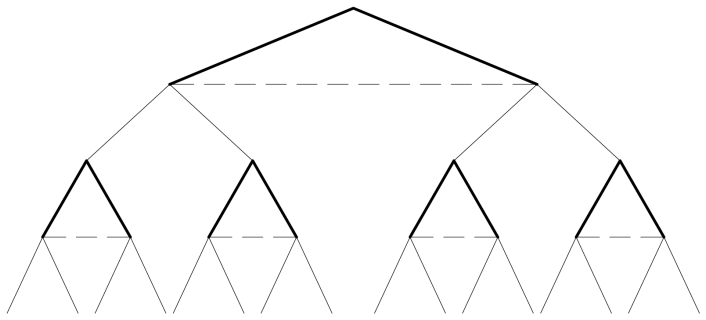
\includegraphics[width=0.75\linewidth]{images/tree3.png}
    \caption{Tree with imperfect information}
\end{figure}
The dashed lines in the figure indicate that a player does not know exactly which vertex they occupy.
\begin{definition}[\textit{Information set}]
    An information set for Player $i$ is a pair $(U_i, A(U_i))$ satisfying the following conditions: 
\end{definition}
\begin{enumerate}
    \item $U_i \subset P_i$ is a non-empty set of vertices $v_1, \cdots, v_k$.
    \item Each vertex $v_j\in U_i$ has the same number of children.
    \item $A_i(U_i)$ is a partition of the children of $v_1 \cup \dots \cup v_k$ such that each element of the partition contains exactly one child from each vertex $v_j$.
\end{enumerate}
Thus, Player $i$ knows they are in $U_i$ but cannot determine the exact vertex.
The partition defines the choice function, indicating that each set in $A_i(U_i)$ corresponds to an available move for the player (graphically, this represents the same choice, or edge, emanating from different vertices).
\begin{definition}[\textit{Extensive form game with imperfect information}]
    An extensive form game with imperfect information is characterized by the following components:
\end{definition}
\begin{enumerate}
    \item A finite set $N = \{1, \dots, n\}$ of players. 
    \item A game tree $(V, E, x_0)$. 
    \item A partition comprising sets $P_1, P_2, \dots, P_{n+1}$ of the non-leaf vertices.
    \item A partition $(U^j_i), j = 1, \dots, ki$ of the set $P_i$, for all $i$, with $(U^j_i, A^j_i)$ being the information set for all players $i$ at all vertices $j$ (having the same number of children). 
    \item A probability distribution defined for each vertex in $P_{n+1}$ on the edges leading to its children.
    \item An $n$-dimensional vector assigned to each leaf.
\end{enumerate}
It is important to note that if the partition consists of only a single vertex, then a game with imperfect information effectively becomes a game with perfect information.
\begin{definition}[\textit{Pure strategy}]
    A pure strategy for player $i$ in an imperfect information game is a function defined over the collection $\mathcal{U}$ of their information sets, assigning to each $U_i\in\mathcal{U}$ an element from the partition $A(U_i)$. 
\end{definition}
\begin{definition}[\textit{Mixed strategy}]
    A mixed strategy is defined as a probability distribution over the pure strategies.
\end{definition}
A game of perfect information is a specific type of imperfect information game where all information sets for all players are singletons.